\section{Random Matrices}

\subsection{Why is a Random Matrix}

%\begin{frame}
%%	\begin{columns}
%%		\begin{column}{0.5\textwidth}
%%			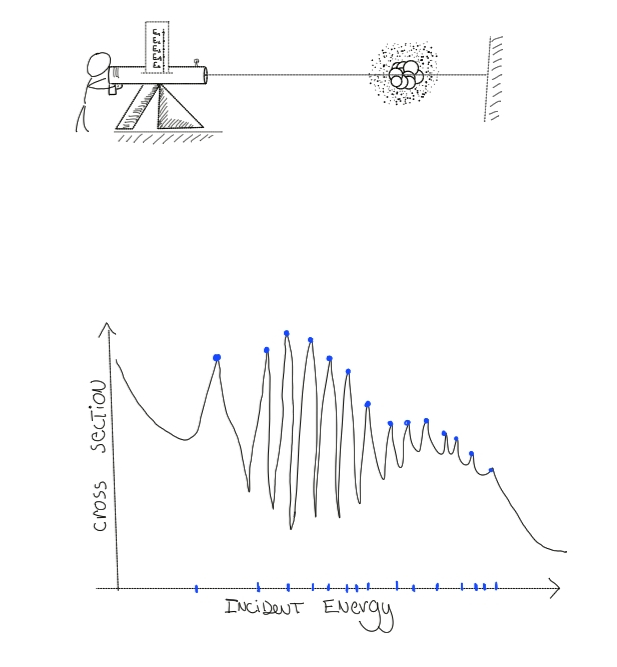
\includegraphics[width=\textwidth]{./media/aesthetics/nuclearscattering.jpg}
%%		\end{column}
%%		\visible<2-3>{
%%			\begin{column}{0.5\textwidth} 
%%				\vspace{1cm}
%%				\begin{equation*}
%%					\Hf \phi_i = E_i \phi_i
%%				\end{equation*}
%%				\visible<3>{
%%					\hspace{0.1cm}
%%					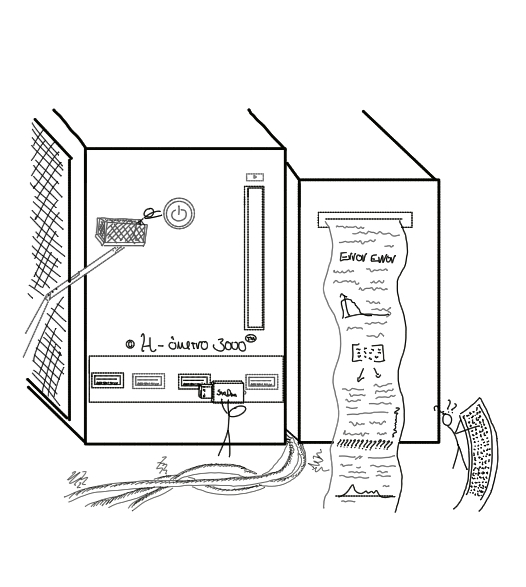
\includegraphics[width=0.8\textwidth]{./media/aesthetics/computer.jpg}
%%				}
%%			\end{column}
%%		}
%%	\end{columns}	
%%	
%\end{frame}

%\begin{frame}
%	\begin{block}{Eugene Wigner - \textit{On the Wigner Surmise} (1956)}
%		``\textit{Perhaps I am now too courageous when I try to guess the distribution of the distances between successive levels (of energies of heavy nuclei) [...] The question is simply what are the distances of the characteristic values of a symmetric matrix with random coefficients.}''
%	\end{block}
%	\vspace{5.5cm}
%	\visible<2-3>{
%		\begin{columns}
%			\begin{column}{0.25\textwidth} 
%				\visible<3>{
%					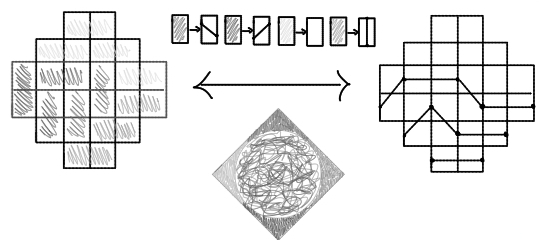
\includegraphics[width=\textwidth]{./media/aesthetics/aztecdiamond.jpg}
%					
%					
\includegraphics[width=\textwidth]{./media/aesthetics/matching.jpg}
%				}
%			\end{column}
%			\begin{column}{0.5\textwidth}
%				\hspace{0.2cm}
%				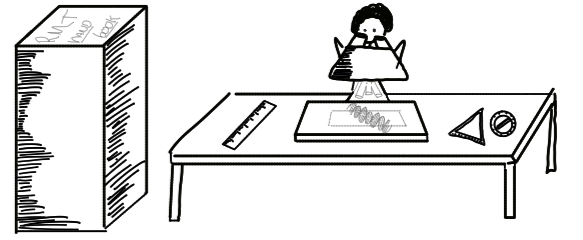
\includegraphics[width=0.9\textwidth]{./media/aesthetics/modelling.jpg}
%			\end{column}
%			\begin{column}{0.25\textwidth} 
%				\visible<3>{
%					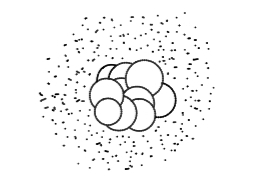
\includegraphics[width=0.8\textwidth]{./media/aesthetics/nucleii.jpg}
%					
%					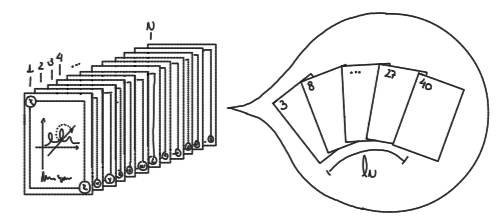
\includegraphics[width=\textwidth]{./media/aesthetics/sequences.jpg}
%				}
%			\end{column}
%		\end{columns}
%	}	
%\end{frame}

{
	\setbeamercolor{background canvas}{bg=}
	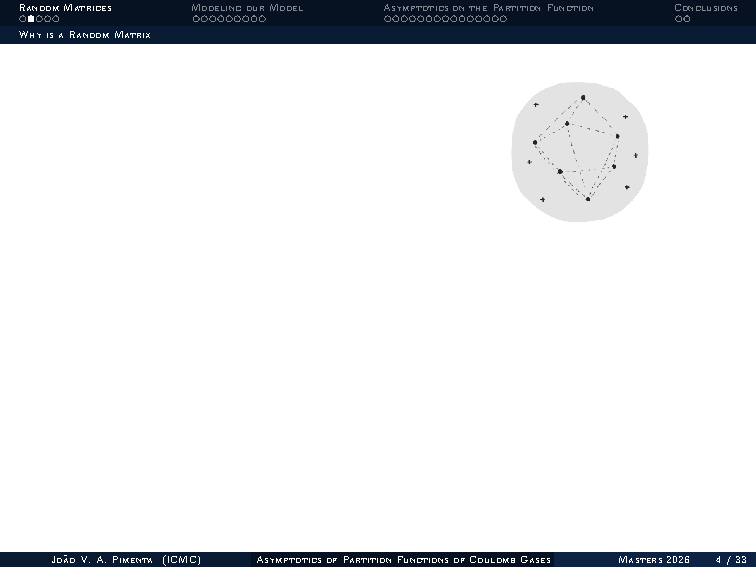
\includepdf[pages={1-}]{why.pdf}
}

\addtocounter{framenumber}{+1}

\subsection{What is a Random Matrix}

\begin{frame}
	\vspace{-0.5cm}
	\only<8->{
		We can think of the matrix itself as a random variable, a measurable map from a probability measure space to $\mathcal{M}_n$.
		\vspace{-0.7cm}
	}
	\only<1-2>{\vspace{-0.25cm}}
	\only<1-7>{
	A \textit{random matrix} is a matrix with \textit{random variables} as entries. 
	}
	\vfill
	\begin{columns}
		\begin{column}{0.5\textwidth}
			\only<1,2>{
				\begin{center}
					$
					\begin{bmatrix}
						x_{1,1} & x_{1,2}& x_{1,3} & x_{1,4}  \\
						x_{2,1} & x_{2,2}& x_{2,3} & x_{2,4} \\
						x_{3,1} & x_{3,2}& x_{3,3} & x_{3,4}  \\
						x_{4,1} & x_{4,2}& x_{4,3} & x_{4,4}  \\
						x_{5,1} & x_{5,2}& x_{5,3} & x_{5,4}
					\end{bmatrix}
					$
				\end{center}
			}
			\only<3>{
				\begin{center}
					$
					\begin{bmatrix}
						-1 & -1 & 1 & 1 \\
						-1 & 1 & -1 & 1 \\
						-1 & 1 & -1 & -1 \\
						-1 & -1 & 1 & -1 \\
						-1 & 1 & -1 & 1 
					\end{bmatrix}
					$
										\vspace{0.5cm}
				\end{center}
			}
			\only<4>{
				\begin{center}
					$
					\begin{bmatrix}
						0.213&0.368&0.912&0.881\\
						0.759&0.692&0.000&0.332\\
						0.898&0.987&0.422&0.623\\
						0.145&0.880&0.522&0.686\\
						0.753&0.687&0.787&0.515
					\end{bmatrix}
					$
										\vspace{0.5cm}
				\end{center}
			}
			\only<5>{
				\begin{center}
					$
					\begin{bmatrix}
						-0.022&-1.340&-0.483&-1.134\\
						1.752&-1.644&1.081&-0.936\\
						-1.058&-0.091&0.544&-0.382\\
						0.633&0.567&0.606&-0.621\\
						-0.316&-1.128&-0.150&0.251
					\end{bmatrix}
					$
					\vspace{0.5cm}
				\end{center}
			}
			\only<6>{
			\begin{center}
				$
				\left[\begin{smallmatrix}
					-2.0+0.1\ii&-0.2-0.9\ii&-0.4-0.3\ii&-0.3+1.0\ii\\
					-1.6-0.8\ii&0.3-0.6\ii&-1.7+0.9\ii&-0.1+0.3\ii\\
					-0.5-0.9\ii&-0.5+0.2\ii&1.2+1.0\ii&0.4-1.3\ii\\
					-0.6+2.4\ii&0.1-0.7\ii&-0.2+1.6\ii&0.6-0.4\ii\\
					0.1-1.3\ii&-0.2-0.9\ii&1.2-1.6\ii&2.1+2.0\ii\\
				\end{smallmatrix}\right]
				$
				\vspace{0.8cm}
			\end{center}
			}
			\only<7-9>{
				\begin{center}
					$
					\left[\begin{smallmatrix}
					-0.8&-0.2-1.5\ii&0.9-0.6\ii&-3.2+2.3\ii \\
					-0.2+1.5\ii&0.5&-1.8-0.8\ii&1.5+1.8\ii \\
					0.9+0.6\ii&-1.8+0.8\ii&1.8&2.1+2.5\ii \\
					-3.2-2.3\ii&1.5-1.8\ii&2.1-2.5\ii&2.4
					\end{smallmatrix}\right]
					$
					\vspace{0.8cm}
				\end{center}
			}
		\end{column}
		\begin{column}{0.5\textwidth}  %%<--- here
			\only<1>{
			\begin{table}
				\centering
				\begin{tabular}{l | c | c }
					$\p(x_{i,j})$ & $\Se$ & $\M_n$ \\
					\hline \hline
					Discrete& $\R$  & General\\ 
					Uniform & $\C$ &  Hermitian \\
					Gaussian & $\mathbb{H}$ & Normal \\
					\vdots  & \vdots  &  \vdots \\
					\hline
				\end{tabular}
			\end{table}
			}
			\only<2>{
				\begin{table}
					\centering
					\begin{tabular}{l | c | c }
						$\p(x_{i,j})$ & $\Se$ & $\M_n$ \\
						\hline \hline
						Discrete& \cellcolor{red!10}$\R$  & \cellcolor{green!10}General\\ 
						Uniform & $\C$ &  Hermitian \\
						Gaussian & $\mathbb{H}$ & Normal \\
						\vdots  & \vdots  &  \vdots \\
						\hline
					\end{tabular}
				\end{table}
			}
			\only<3>{
				\begin{table}
					\centering
					\begin{tabular}{l | c | c }
						$\p(x_{i,j})$ & $\Se$ & $\M_n$ \\
						\hline \hline
						\cellcolor{blue!10} Discrete& \cellcolor{red!10}$\R$  & \cellcolor{green!10}General\\ 
						Uniform & $\C$ &  Hermitian \\
						Gaussian & $\mathbb{H}$ & Normal \\
						\vdots  & \vdots  &  \vdots \\
						\hline
						\multicolumn{3}{c}{	\fcolorbox{white}{blue!10}{} \!\!\!\! \fcolorbox{white}{red!10}{}  \!\!\!\! \fcolorbox{white}{green!10}{}}
					\end{tabular}
				\end{table}
			}
			\only<4>{
				\begin{table}
					\centering
					\begin{tabular}{l | c | c }
						$\p(x_{i,j})$ & $\Se$ & $\M_n$ \\
						\hline \hline
						Discrete& \cellcolor{red!10}$\R$  & \cellcolor{green!10}General\\ 
						\cellcolor{blue!10}Uniform & $\C$ &  Hermitian \\
						Gaussian & $\mathbb{H}$ & Normal \\
						\vdots  & \vdots  &  \vdots \\
						\hline
						\multicolumn{3}{c}{	\fcolorbox{white}{blue!10}{} \!\!\!\! \fcolorbox{white}{red!10}{}  \!\!\!\! \fcolorbox{white}{green!10}{}} \\
					\end{tabular}
				\end{table}
			}
			\only<5>{
				\begin{table}
					\centering
					\begin{tabular}{l | c | c }
						$\p(x_{i,j})$ & $\Se$ & $\M_n$ \\
						\hline \hline
						Discrete& \cellcolor{red!10}$\R$  & \cellcolor{green!10}General\\ 
						Uniform & $\C$ &  Hermitian \\
						\cellcolor{blue!10}Gaussian & $\mathbb{H}$ & Normal \\
						\vdots  & \vdots  &  \vdots \\
						\hline
						\multicolumn{3}{c}{	\fcolorbox{white}{blue!10}{} \!\!\!\! \fcolorbox{white}{red!10}{}  \!\!\!\! \fcolorbox{white}{green!10}{}} \\
						\multicolumn{3}{c}{ 
							Ginibre Orthogonal Ensemble} 
					\end{tabular}
				\end{table}
			}
			\only<6>{
				\begin{table}
					\centering
					\begin{tabular}{l | c | c }
						$\p(x_{i,j})$ & $\Se$ & $\M_n$ \\
						\hline \hline
						Discrete& $\R$  & \cellcolor{green!10}General\\ 
						Uniform & \cellcolor{red!10}$\C$ &  Hermitian \\
						\cellcolor{blue!10}Gaussian & $\mathbb{H}$ & Normal \\
						\vdots  & \vdots  &  \vdots \\
						\hline
						\multicolumn{3}{c}{	\fcolorbox{white}{blue!10}{} \!\!\!\! \fcolorbox{white}{red!10}{}  \!\!\!\! \fcolorbox{white}{green!10}{}} \\
						\multicolumn{3}{c}{ 
							Ginibre Unitary Ensemble} 
					\end{tabular}
				\end{table}
			}
			\only<7-8>{
				\begin{table}
					\centering
					\begin{tabular}{l | c | c }
						$\p(x_{i,j})$ & $\Se$ & $\M_n$ \\
						\hline \hline
						Discrete& $\R$  & General\\ 
						Uniform & \cellcolor{red!10}$\C$ &  \cellcolor{green!10}Hermitian \\
						\cellcolor{blue!10}Gaussian & $\mathbb{H}$ & Normal \\
						\vdots  & \vdots  &  \vdots \\
						\hline
						\multicolumn{3}{c}{	\fcolorbox{white}{blue!10}{} \!\!\!\! \fcolorbox{white}{red!10}{}  \!\!\!\! \fcolorbox{white}{green!10}{}} \\
						\multicolumn{3}{c}{ 
							Gaussian Unitary Ensemble} 
					\end{tabular}
				\end{table}
			}
			\only<9>{
			\vspace{-0.15cm}
				\begin{table}
					\centering
					\begin{tabular}{l | c | c }
						$\eP(\m{X})$ & $\Se$ & $\M_n$ \\
						\hline \hline
						\cellcolor{blue!10}$\ee^{-n \tr(\m{X}^2)}$ &$\R$  & General\\ 
						$\ee^{-n \tr{(\m{X}^* \m{X})}}$ &  \cellcolor{red!10}$\C$ &  \cellcolor{green!10}Hermitian \\
						$\ee^{-n \tr{(Q(\m{X}))}}$ & $\mathbb{H}$ & Normal \\
						\vdots  & \vdots  &  \vdots \\
						\hline
						\multicolumn{3}{c}{	\fcolorbox{white}{blue!10}{} \!\!\!\! \fcolorbox{white}{red!10}{}  \!\!\!\! \fcolorbox{white}{green!10}{}} \\
						\multicolumn{3}{c}{Gaussian Unitary Ensemble} 
					\end{tabular}
				\end{table}
			\vspace{-0.15cm}
			}
		\end{column}
	\end{columns}
	\vfill
	\only<1-3>{
		\visible<3>{
		\begin{equation*}
			\eP(\m{X}) = \prod_{i,j=1}^{n} p(x_{i,j}) = U^{n^2}(\{-1, 1\})
		\end{equation*}
		}
    }
	\only<4>{
		\begin{equation*}
			\eP(\m{X}) = \prod_{i,j=1}^{n} p(x_{i,j}) = U^{n^2}([0,1])
		\end{equation*}
	}
	\only<5>{
		\begin{equation*}
			\eP(\m{X}) = \prod_{i,j=1}^{n} \ee^{-n x_{i,j}^2}
		\end{equation*}
	}
	\only<6>{
		\begin{equation*}
			\eP(\m{X}) = \prod_{i,j=1}^{n} \ee^{-n x_{i,j}^2} \ee^{-n y_{i,j}^2}
		\end{equation*}
	}
	\only<7-8>{
		\begin{equation*}
			\eP(\m{X}) = \prod_{i=1}^{n} \ee^{-n z_{i,j}^2} \prod_{i>j}^{n} \ee^{-2n |z_{i,j}|^2}
		\end{equation*}
	}
	\only<9>{
		\begin{equation*}
			\eP(\m{X}) = \prod_{i=1}^{n} \ee^{-n z_{i,j}^2} \prod_{i>j}^{n} \ee^{-2n |z_{i,j}|^2} \propto \ee^{-n \tr(\m{X}^2)}
		\end{equation*}
	}
\end{frame}

\subsection{Normal Matrix Density}

\begin{frame}
	\only<1->{\vspace{0.1cm}}
	\only<1->{
	We can think of the matrix itself as a random variable, a measurable map from a probability measure space to $\mathcal{M}_n$.
	}
	\begin{columns}
		\begin{column}{0.5\textwidth}
		\only<2-3>{
			Normal matrices are similar to diagonal matrices, i.e.
			\begin{equation*}
				\m{X} = \m{U} \m{\Lambda} \m{U}^*.
			\end{equation*}
			Moreover, the spectra is typically simple. 
		}
		\only<4->{
			Invariance by unitary conjugation means independence of coordinates. 
			\begin{equation*}
				\dd\eP(\m{X}_1) = \dd\eP(\m{X}_2) \iff \m{X}_1 = \m{U} \m{X}_2 \m{U}^*
			\end{equation*}
			for some unitary $U$.
		}
		\end{column}
		\begin{column}{0.5\textwidth}  %%<--- here
		\only<1-5>{
			\begin{table}
				\centering
				\begin{tabular}{l | c | c }
					$\eP(\m{X})$ & $\Se$ & $\M_n$ \\
					\hline \hline
					$\ee^{-n \tr(\m{X}^2)}$ &$\R$  & General\\ 
					$\ee^{-n \tr{(\m{X}^* \m{X})}}$ &  \cellcolor{red!10}$\C$ &  Hermitian \\
					$\ee^{-n \tr{(Q(\m{X}))}}$ & $\mathbb{H}$ & \cellcolor{green!10}Normal \\
					\vdots  & \vdots  &  \vdots \\
					\hline
					\multicolumn{3}{c}{ \fcolorbox{white}{red!10}{}  \!\!\!\! \fcolorbox{white}{green!10}{}} \\
				\end{tabular}
			\end{table}
		}
		\only<6->{
			\begin{table}
				\centering
				\begin{tabular}{l | c | c }
					$\eP(\m{X})$ & $\Se$ & $\M_n$ \\
					\hline \hline
					$\ee^{-n \tr(\m{X}^2)}$ &$\R$  & General\\ 
					$\ee^{-n \tr{(\m{X}^* \m{X})}}$ &  \cellcolor{red!10}$\C$ &  Hermitian \\
					\cellcolor{blue!10}$\ee^{-n \tr{(Q(\m{X}))}}$ & $\mathbb{H}$ & \cellcolor{green!10}Normal \\
					\vdots  & \vdots  &  \vdots \\
					\hline
					\multicolumn{3}{c}{	\fcolorbox{white}{blue!10}{} \!\!\!\! \fcolorbox{white}{red!10}{}  \!\!\!\! \fcolorbox{white}{green!10}{}} \\
				\end{tabular}
			\end{table}
		}
		\end{column}
	\end{columns}
	\visible<2->{
		\only<5->{
			We want that $\dd \eP(\m{X}) = \eP(\m{X}) \dd \m{X}$ is invariant.
		}
		\only<1-2>{
			\vspace{3.27cm}
		}
		\only<5,6>{
			\vspace{2.8cm}
		}
		\only<3-4>{
			\begin{equation*}
				\m{X} \mapsto (\m{\Lambda}, \m{U}) = \left(
					\begin{tikzpicture}[baseline=8ex, scale=0.70]
					\begin{axis}[axis line style={opacity=1}, ticks=none,
						xmin=-1.5, xmax=1.5,
						ymin=-1.5, ymax=1.5,
						axis x line=middle,
						axis y line=middle,
						xticklabel=\empty,
						yticklabel=\empty,
						xticklabel pos=top,
						xlabel=$\R$,
						ylabel=$\ii \R$,
						scatter/classes={%
							a={ mark size=0.5pt}}
						]
						\addplot[skip coords between index={10}{500}, opacity=1, scatter, mark=x, black, only marks] table [col sep=comma] {./media/aesthetics/5lines/a2t0.csv};
					\end{axis}
				\end{tikzpicture} \hspace{0.3cm},
				\begin{tikzpicture}[baseline=0ex, line cap=round]
					\coordinate (O) at (0,0);
					\coordinate (A) at ( -5:1.1);
					\coordinate (B) at ( 55:1.4);
					\coordinate (C) at (130:1.2);
					\coordinate (D) at (210:2.0);
					\coordinate (E) at (65:1.60);
					\coordinate (F) at (-110:1.2);
					\coordinate (G) at (30:1.3);
					\coordinate (H) at (200:1.2);
					\coordinate (I) at (-30:1.4);
					\coordinate (J) at (123:0.4);
					\draw[vector,black] (O) -- (A) node[right=-2] {};
					\draw[vector,black] (O) -- (B) node[above right=-3] {};
					\draw[vector,black] (O) -- (C) node[above left=-3] {};
					\draw[vector,black] (O) -- (D) node[left=-1] {};
					\draw[vector,black] (O) -- (E) node[left=-1] {};
					\draw[vector,black] (O) -- (F) node[left=-1] {};
					\draw[vector,black] (O) -- (G) node[left=-1] {};
					\draw[vector,black] (O) -- (H) node[left=-1] {};
					\draw[vector,black] (O) -- (I) node[left=-1] {};
					\draw[vector,black] (O) -- (J) node[left=-1] {};
				\end{tikzpicture} \hspace{-1cm}
				\right)
			\end{equation*}
%	\begin{columns}
%		\begin{column}{0.1\textwidth}  %%<--- here
%			\begin{center}
%				$ \m{X} \mapsto
%				$
%			\end{center}
%		\end{column}
%		\begin{column}{0.4\textwidth}  %%<--- here
%			\begin{center}
%				\begin{tikzpicture}[scale=0.70]
%					\begin{axis}[axis line style={opacity=1}, ticks=none,
%						xmin=-1.5, xmax=1.5,
%						ymin=-1.5, ymax=1.5,
%						axis x line=middle,
%						axis y line=middle,
%						xticklabel=\empty,
%						yticklabel=\empty,
%						xticklabel pos=top,
%						xlabel=$\R$,
%						ylabel=$\ii \R$,
%						scatter/classes={%
%							a={ mark size=0.5pt}}
%						]
%						\addplot[skip coords between index={10}{500}, opacity=1, scatter, mark=x, black, only marks] table [col sep=comma] {./media/aesthetics/5lines/a2t0.csv};
%					\end{axis}
%				\end{tikzpicture}
%			\end{center}
%		\end{column}
%		\begin{column}{0.4\textwidth}
%			\begin{center}
%				\begin{tikzpicture}[line cap=round]
%					\coordinate (O) at (0,0);
%					\coordinate (A) at ( -5:1.1);
%					\coordinate (B) at ( 55:1.4);
%					\coordinate (C) at (130:1.2);
%					\coordinate (D) at (210:2.0);
%					\coordinate (E) at (65:1.60);
%					\coordinate (F) at (-110:1.2);
%					\coordinate (G) at (30:1.3);
%					\coordinate (H) at (200:1.2);
%					\coordinate (I) at (-30:1.4);
%					\coordinate (J) at (123:0.4);
%					\draw[vector,black] (O) -- (A) node[right=-2] {};
%					\draw[vector,black] (O) -- (B) node[above right=-3] {};
%					\draw[vector,black] (O) -- (C) node[above left=-3] {};
%					\draw[vector,black] (O) -- (D) node[left=-1] {};
%					\draw[vector,black] (O) -- (E) node[left=-1] {};
%					\draw[vector,black] (O) -- (F) node[left=-1] {};
%					\draw[vector,black] (O) -- (G) node[left=-1] {};
%					\draw[vector,black] (O) -- (H) node[left=-1] {};
%					\draw[vector,black] (O) -- (I) node[left=-1] {};
%					\draw[vector,black] (O) -- (J) node[left=-1] {};
%				\end{tikzpicture}
%			\end{center}
%		\end{column}
%	\end{columns}
		}
	\only<7>{
	\vspace{0.1cm}
	\begin{align*}
		\exp\left(-n\tr{Q(\m{U}\m{X_1}\m{U}^*)}\right) &= \exp\left(-n\tr{Q(\m{U}^*\m{U}\m{X_1})}\right) = \exp\left(-n\tr{Q(\m{X_1})}\right) \\ & = \exp\left(-n\tr{Q(\m{U}\m{\Lambda}\m{U}^*)}\right) = \exp\left(-n\sum_i^n {Q(\lambda_i)} \right).
	\end{align*}
	\vspace{0.1cm}
	}
	\only<8>{
	\begin{equation*}
		\dd \m{X} = \prod_{1 \leq i < j \leq n} |z_i - z_j|^2 \prod_{i=1}^{n} \dd^2 z_i  \dd \m{U} ,
	\end{equation*}
	where $\dd \m{U}$ is the Haar measure on eigenvectors and $\dd^2 z$ is Lebesgue measure on $\C$.
	\vspace{0.5cm}
	}
	}
\end{frame}

%\begin{frame}
%	\begin{theorem}	
%	\label{Theorem: Weyls}
%	\textit{(Weyl's integration formula - Unitary case)} 
%	The measure $\dd \m{X}$ decomposes almost everywhere in $\mathcal{N}(\C)$ as 
%	\begin{equation*}
%		\dd \m{X} = \dd \m{U} \prod_{1 \leq i < j \leq n} |z_i - z_j|^2  \prod_{i=1}^{n} \dd^2 z_i,
%	\end{equation*}
%	where $\{z_i\}_{i=1}{n}$ is the spectrum of $\m{X}$, $\m{M} = \m{U} \m{\Lambda} \m{U}^*$ for $\m{\Lambda} =\diag\{z_i\}_{i=1}^n$, $\m{U} \in U(n)/U(1)^n$ and the measure
%	\begin{equation*}
%		\dd \m{U} = 2^{\frac{n(n-1)}{4}} \prod_{i<j} \dd^2 u_{i,j}, \quad \dd^2 u_{i,j} = (\m{U}^*)_{i,k}\dd^2\m{U}_{k,j}
%	\end{equation*}
%	on $U(n)/U(1)^n$ is induced by the measure on $U(n)$ and is a Haar measure.
%\end{theorem}
%\end{frame}

\begin{frame}
	We set the ensemble
	\begin{equation*}
		\eE = (\eS, \eP) \quad \text{with} \quad 
		\begin{cases}
			\eS = \mathcal{N}_n(\C) \\
			\eP(\m{X}) = \exp\left\{- n \tr(Q(\m{X}))\right\}
		\end{cases}
	\end{equation*}
	such that 
	\begin{equation*}
		\dd \eP(\m{X}) = \prod_ {i < j}^n |z_i - z_j|^2 \prod_{j=1}^{n} \ee^{- n \Q(z_j)} \dd^2 z_j \dd \m{U}.
	\end{equation*}
	\visible<2->{
	\begin{align*}
		\int_{\mathcal{M}_n} \dd \eP(\m{X}) & = \int_{\C^n} \int_{\tilde{U}(n)}  \prod_ {i < j}^n |z_i - z_j|^2 \prod_{j=1}^{n} \ee^{- n \Q(z_j)} \dd^2 z_j \dd \m{U} \\ & = \int_{\C^n} \frac{\prod_ {i < j}^n |z_i - z_j|^2 \prod_{j=1}^{n} \ee^{- n \Q(z_j)}}{\pZ{n}{Q}}  \dd^2 z_j
	\end{align*}
} \visible<3->{ we have
	\begin{equation*}
		p_n(\{z_i\}_{i=1}^n) = \frac{1}{\pZ{n}{Q}} \prod_ {i < j}^n |z_i - z_j|^2 \prod_{j=1}^{n} \ee^{- n \Q(z_j)} 
	\end{equation*}
}
\end{frame}
%---------------------------------------------------------
